\documentclass[border=3mm]{standalone}
\usepackage{tikz}
\usetikzlibrary{arrows.meta,positioning,shapes.geometric,shapes.misc,fit,calc,backgrounds,decorations.pathreplacing,patterns}
\usepackage{amsmath,amssymb}

% ==============================================================================
% Coordinated Palette (Aligned with Figure 1)
% ==============================================================================
\definecolor{cSystem}{HTML}{1A5276}   % Slate Blue: Telemetry
\definecolor{cChaos}{HTML}{D35400}    % Rich Amber/Orange: Threat Modulation
\definecolor{cPolicy}{HTML}{5B2C6F}   % Deep Purple/Violet: Neural Policy & Controller
\definecolor{cMitig}{HTML}{196F3D}    % Emerald Green: Actions & Value
\definecolor{cRisk}{HTML}{922B21}     % Deep Crimson: Security Risks
\definecolor{cAux}{HTML}{C0392B}      % Auxiliary Loss Crimson
\definecolor{cBorder}{HTML}{7F8C8D}   % Boundary Framing

\begin{document}
\sffamily\footnotesize
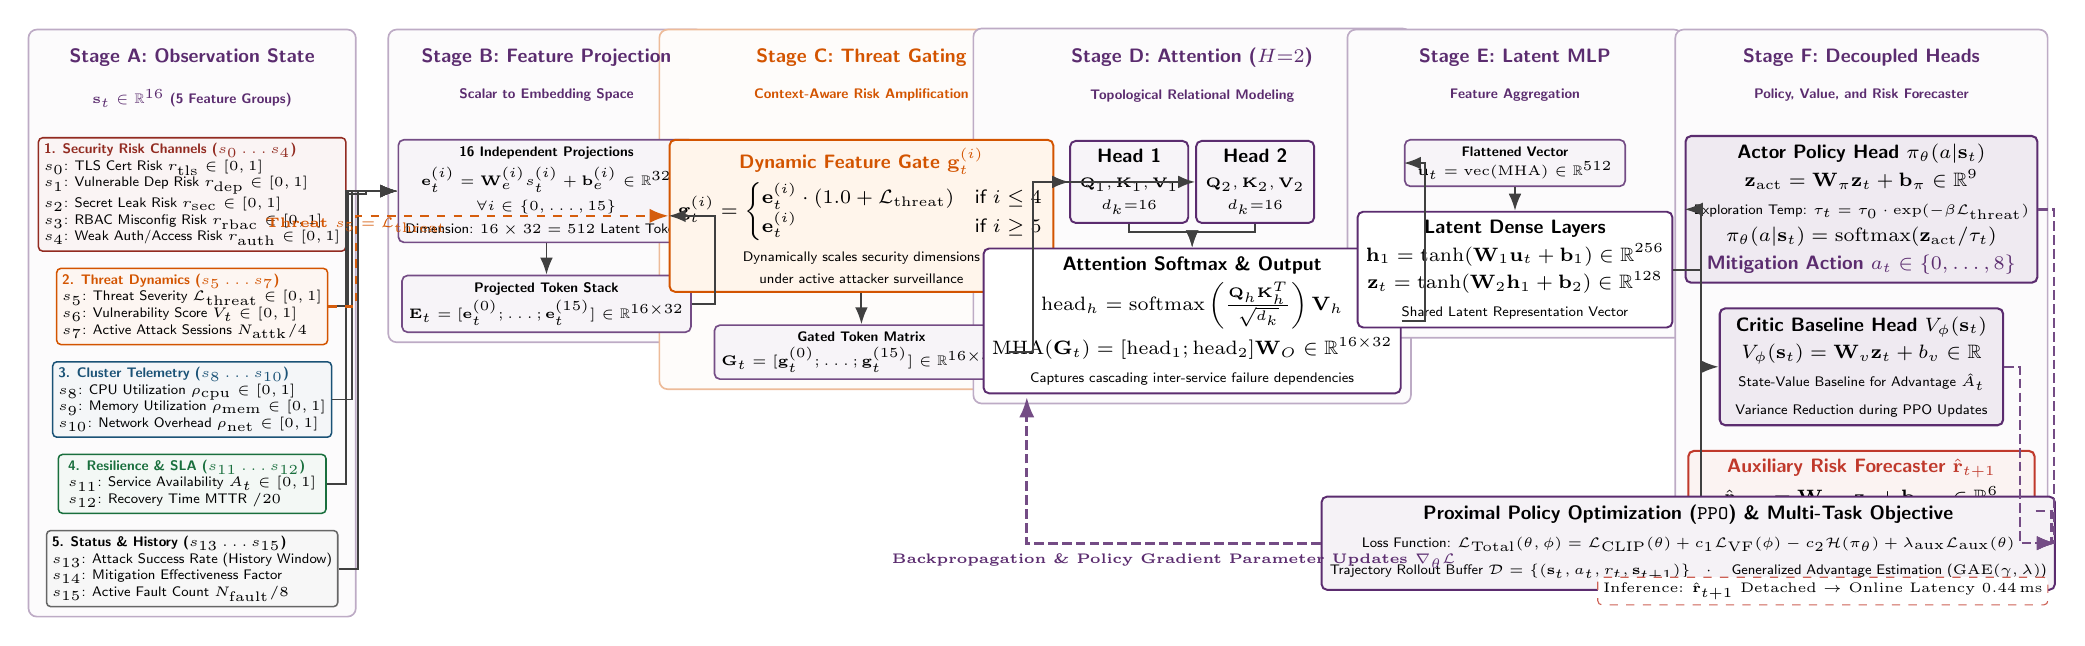
\begin{tikzpicture}[
    >=Latex,
    font=\sffamily,
    featpill/.style={
        draw=black!70, line width=0.55pt, fill=white,
        rounded corners=1.5pt, inner sep=2pt, align=left,
        font=\sffamily\tiny, minimum width=34mm
    },
    transcard/.style={
        draw=cPolicy!85, line width=0.6pt, fill=cPolicy!5,
        rounded corners=2pt, inner sep=2.5pt, align=center,
        font=\sffamily\tiny, minimum width=28mm
    },
    opcard/.style={
        draw=cPolicy, line width=0.7pt, fill=white,
        rounded corners=2pt, inner sep=3pt, align=center,
        font=\sffamily\scriptsize
    },
    headcard/.style={
        draw=cPolicy, line width=0.75pt, fill=cPolicy!10,
        rounded corners=2pt, inner sep=3pt, align=center,
        font=\sffamily\scriptsize
    },
    sigflow/.style={
        ->, line width=0.7pt, draw=black!75
    },
    modflow/.style={
        ->, dashed, line width=0.85pt, draw=cChaos!95
    },
    optflow/.style={
        ->, line width=0.85pt, draw=cPolicy!85, dash pattern=on 3.5pt off 1.5pt
    }
]

% ==============================================================================
% STAGE A: OBSERVATION INPUT VECTOR (s_t in R^16)
% ==============================================================================
\node[font=\sffamily\bfseries\scriptsize, text=cPolicy] (hdrA) at (0, 8.2) {Stage A: Observation State};
\node[font=\sffamily\bfseries\tiny, text=cPolicy, below=0.5mm of hdrA] (subA) {$\mathbf{s}_t \in \mathbb{R}^{16}$ (5 Feature Groups)};

% Group 1: Security Risks (s0 - s4)
\node[featpill, draw=cRisk, fill=cRisk!5, below=2.5mm of subA] (g_risk) {
    \textbf{\textcolor{cRisk}{1. Security Risk Channels ($s_0\dots s_4$)}}\\
    $s_0$: TLS Cert Risk $r_{\mathrm{tls}} \in [0, 1]$\\
    $s_1$: Vulnerable Dep Risk $r_{\mathrm{dep}} \in [0, 1]$\\
    $s_2$: Secret Leak Risk $r_{\mathrm{sec}} \in [0, 1]$\\
    $s_3$: RBAC Misconfig Risk $r_{\mathrm{rbac}} \in [0, 1]$\\
    $s_4$: Weak Auth/Access Risk $r_{\mathrm{auth}} \in [0, 1]$
};

% Group 2: Threat & Adversary Dynamics (s5 - s7)
\node[featpill, draw=cChaos, fill=cChaos!5, below=2mm of g_risk] (g_threat) {
    \textbf{\textcolor{cChaos}{2. Threat Dynamics ($s_5\dots s_7$)}}\\
    $s_5$: Threat Severity $\mathcal{L}_{\mathrm{threat}} \in [0, 1]$\\
    $s_6$: Vulnerability Score $V_t \in [0, 1]$\\
    $s_7$: Active Attack Sessions $N_{\mathrm{attk}} / 4$
};

% Group 3: Cluster Resource Telemetry (s8 - s10)
\node[featpill, draw=cSystem, fill=cSystem!5, below=2mm of g_threat] (g_telemetry) {
    \textbf{\textcolor{cSystem}{3. Cluster Telemetry ($s_8\dots s_{10}$)}}\\
    $s_8$: CPU Utilization $\rho_{\mathrm{cpu}} \in [0, 1]$\\
    $s_9$: Memory Utilization $\rho_{\mathrm{mem}} \in [0, 1]$\\
    $s_{10}$: Network Overhead $\rho_{\mathrm{net}} \in [0, 1]$
};

% Group 4: Resilience QoS & Recovery (s11 - s12)
\node[featpill, draw=cMitig, fill=cMitig!5, below=2mm of g_telemetry] (g_qos) {
    \textbf{\textcolor{cMitig}{4. Resilience \& SLA ($s_{11}\dots s_{12}$)}}\\
    $s_{11}$: Service Availability $A_t \in [0, 1]$\\
    $s_{12}$: Recovery Time MTTR $/ 20$
};

% Group 5: History & Fault Status (s13 - s15)
\node[featpill, draw=black!60, fill=black!3, below=2mm of g_qos] (g_hist) {
    \textbf{5. Status \& History ($s_{13}\dots s_{15}$)}\\
    $s_{13}$: Attack Success Rate (History Window)\\
    $s_{14}$: Mitigation Effectiveness Factor\\
    $s_{15}$: Active Fault Count $N_{\mathrm{fault}} / 8$
};

% Frame for Stage A
\begin{scope}[on background layer]
    \node[draw=cPolicy!40, line width=0.6pt, fill=cPolicy!2, rounded corners=3pt,
          fit=(hdrA) (subA) (g_risk) (g_hist)] (boxA) {};
\end{scope}

% ==============================================================================
% STAGE B: LINEAR FEATURE PROJECTION
% ==============================================================================
\node[font=\sffamily\bfseries\scriptsize, text=cPolicy] (hdrB) at (4.5, 8.2) {Stage B: Feature Projection};
\node[font=\sffamily\bfseries\tiny, text=cPolicy, below=0.5mm of hdrB] (subB) {Scalar to Embedding Space};

% 16 Independent Embeddings
\node[transcard, below=3.5mm of subB, minimum width=29mm] (proj_block) {
    \textbf{16 Independent Projections}\\[2pt]
    $\mathbf{e}_t^{(i)} = \mathbf{W}_e^{(i)} s_t^{(i)} + \mathbf{b}_e^{(i)} \in \mathbb{R}^{32}$\\[2pt]
    $\forall i \in \{0, \dots, 15\}$\\[2pt]
    \tiny Dimension: $16 \times 32 = 512$ Latent Tokens
};

% Output representation
\node[transcard, below=4mm of proj_block, minimum width=29mm] (emb_stack) {
    \textbf{Projected Token Stack}\\[1pt]
    $\mathbf{E}_t = [\mathbf{e}_t^{(0)}; \dots; \mathbf{e}_t^{(15)}] \in \mathbb{R}^{16 \times 32}$
};

\draw[sigflow] (proj_block) -- (emb_stack);

% Connect Stage A to Stage B
\draw[sigflow] (g_risk.east) -- ++(0.25, 0) |- (proj_block.west);
\draw[sigflow] (g_threat.east) -- ++(0.25, 0) |- (proj_block.west);
\draw[sigflow] (g_telemetry.east) -- ++(0.25, 0) |- (proj_block.west);
\draw[sigflow] (g_qos.east) -- ++(0.25, 0) |- (proj_block.west);
\draw[sigflow] (g_hist.east) -- ++(0.25, 0) |- (proj_block.west);

% Frame for Stage B
\begin{scope}[on background layer]
    \node[draw=cPolicy!40, line width=0.6pt, fill=cPolicy!2, rounded corners=3pt,
          fit=(hdrB) (subB) (proj_block) (emb_stack)] (boxB) {};
\end{scope}

% ==============================================================================
% STAGE C: THREAT-AWARE FEATURE GATING
% ==============================================================================
\node[font=\sffamily\bfseries\scriptsize, text=cChaos] (hdrC) at (8.5, 8.2) {Stage C: Threat Gating};
\node[font=\sffamily\bfseries\tiny, text=cChaos, below=0.5mm of hdrC] (subC) {Context-Aware Risk Amplification};

% Gating Multiplier Unit
\node[opcard, draw=cChaos, fill=orange!8, below=3.5mm of subC, minimum width=32mm] (gating_node) {
    \textbf{\textcolor{cChaos}{Dynamic Feature Gate $\mathbf{g}_t^{(i)}$}}\\[2pt]
    $\mathbf{g}_t^{(i)} = \begin{cases}
    \mathbf{e}_t^{(i)} \cdot \left(1.0 + \mathcal{L}_{\mathrm{threat}}\right) & \text{if } i \le 4 \\
    \mathbf{e}_t^{(i)} & \text{if } i \ge 5
    \end{cases}$\\[3pt]
    \tiny Dynamically scales security dimensions\\
    \tiny under active attacker surveillance
};

% Gated Token Output
\node[transcard, below=4mm of gating_node, minimum width=32mm] (gated_stack) {
    \textbf{Gated Token Matrix}\\[1pt]
    $\mathbf{G}_t = [\mathbf{g}_t^{(0)}; \dots; \mathbf{g}_t^{(15)}] \in \mathbb{R}^{16 \times 32}$
};

\draw[sigflow] (gating_node) -- (gated_stack);
\draw[sigflow] (emb_stack.east) -- ++(0.3, 0) |- (gating_node.west);

% Threat modulation flow from s5
\draw[modflow] (g_threat.east) -- ++(0.35, 0) |- (gating_node.west)
    node[pos=0.35, above, font=\tiny\bfseries, text=cChaos] {Threat $s_5 = \mathcal{L}_{\mathrm{threat}}$};

% Frame for Stage C
\begin{scope}[on background layer]
    \node[draw=cChaos!40, line width=0.6pt, fill=cChaos!2, rounded corners=3pt,
          fit=(hdrC) (subC) (gating_node) (gated_stack)] (boxC) {};
\end{scope}

% ==============================================================================
% STAGE D: MULTI-HEAD SELF-ATTENTION (H = 2)
% ==============================================================================
\node[font=\sffamily\bfseries\scriptsize, text=cPolicy] (hdrD) at (12.7, 8.2) {Stage D: Attention ($H{=}2$)};
\node[font=\sffamily\bfseries\tiny, text=cPolicy, below=0.5mm of hdrD] (subD) {Topological Relational Modeling};

% Parallel Head 1 & Head 2
\node[opcard, draw=cPolicy, fill=cPolicy!5, below=3.5mm of subD, xshift=-8mm, minimum width=15mm] (attn_h1) {
    \textbf{\scriptsize Head 1}\\[1pt]
    \tiny $\mathbf{Q}_1, \mathbf{K}_1, \mathbf{V}_1$\\
    \tiny $d_k{=}16$
};
\node[opcard, draw=cPolicy, fill=cPolicy!5, below=3.5mm of subD, xshift=8mm, minimum width=15mm] (attn_h2) {
    \textbf{\scriptsize Head 2}\\[1pt]
    \tiny $\mathbf{Q}_2, \mathbf{K}_2, \mathbf{V}_2$\\
    \tiny $d_k{=}16$
};

% Attention Output & Projection
\node[opcard, draw=cPolicy, fill=white, below=3mm of attn_h1, xshift=8mm, minimum width=32mm] (mha_merge) {
    \textbf{Attention Softmax \& Output}\\[2pt]
    $\mathrm{head}_h = \mathrm{softmax}\left(\frac{\mathbf{Q}_h \mathbf{K}_h^T}{\sqrt{d_k}}\right) \mathbf{V}_h$\\[2pt]
    $\mathrm{MHA}(\mathbf{G}_t) = [\mathrm{head}_1; \mathrm{head}_2]\mathbf{W}_O \in \mathbb{R}^{16 \times 32}$\\[2pt]
    \tiny Captures cascading inter-service failure dependencies
};

\draw[sigflow] (gated_stack.east) -- ++(0.3, 0) |- (attn_h1.west);
\draw[sigflow] (gated_stack.east) -- ++(0.3, 0) |- (attn_h2.west);
\draw[sigflow] (attn_h1.south) -- ++(0, -0.1) -| (mha_merge.north);
\draw[sigflow] (attn_h2.south) -- ++(0, -0.1) -| (mha_merge.north);

% Frame for Stage D
\begin{scope}[on background layer]
    \node[draw=cPolicy!40, line width=0.6pt, fill=cPolicy!2, rounded corners=3pt,
          fit=(hdrD) (subD) (attn_h1) (attn_h2) (mha_merge)] (boxD) {};
\end{scope}

% ==============================================================================
% STAGE E: LATENT REPRESENTATION (MLP: 512 -> 256 -> 128)
% ==============================================================================
\node[font=\sffamily\bfseries\scriptsize, text=cPolicy] (hdrE) at (16.8, 8.2) {Stage E: Latent MLP};
\node[font=\sffamily\bfseries\tiny, text=cPolicy, below=0.5mm of hdrE] (subE) {Feature Aggregation};

% Flattening Node
\node[transcard, below=3.5mm of subE, minimum width=28mm] (flatten_node) {
    \textbf{Flattened Vector}\\[1pt]
    $\mathbf{u}_t = \mathrm{vec}(\mathrm{MHA}) \in \mathbb{R}^{512}$
};

% Dense Layers
\node[opcard, draw=cPolicy, fill=white, below=3mm of flatten_node, minimum width=28mm] (dense_layers) {
    \textbf{Latent Dense Layers}\\[2pt]
    $\mathbf{h}_1 = \tanh(\mathbf{W}_1 \mathbf{u}_t + \mathbf{b}_1) \in \mathbb{R}^{256}$\\[2pt]
    $\mathbf{z}_t = \tanh(\mathbf{W}_2 \mathbf{h}_1 + \mathbf{b}_2) \in \mathbb{R}^{128}$\\[2pt]
    \tiny Shared Latent Representation Vector
};

\draw[sigflow] (mha_merge.east) -- ++(0.3, 0) |- (flatten_node.west);
\draw[sigflow] (flatten_node) -- (dense_layers);

% Frame for Stage E
\begin{scope}[on background layer]
    \node[draw=cPolicy!40, line width=0.6pt, fill=cPolicy!2, rounded corners=3pt,
          fit=(hdrE) (subE) (flatten_node) (dense_layers)] (boxE) {};
\end{scope}

% ==============================================================================
% STAGE F: THREE MULTI-TASK DECOUPLED OUTPUT HEADS
% ==============================================================================
\node[font=\sffamily\bfseries\scriptsize, text=cPolicy] (hdrF) at (21.2, 8.2) {Stage F: Decoupled Heads};
\node[font=\sffamily\bfseries\tiny, text=cPolicy, below=0.5mm of hdrF] (subF) {Policy, Value, and Risk Forecaster};

% Head 1: Actor Policy
\node[headcard, below=3mm of subF, minimum width=36mm] (actor_head) {
    \textbf{Actor Policy Head $\pi_\theta(a|\mathbf{s}_t)$}\\[2pt]
    $\mathbf{z}_{\mathrm{act}} = \mathbf{W}_\pi \mathbf{z}_t + \mathbf{b}_\pi \in \mathbb{R}^9$\\[2pt]
    \tiny Exploration Temp: $\tau_t = \tau_0 \cdot \exp(-\beta \mathcal{L}_{\mathrm{threat}})$\\[2pt]
    $\pi_\theta(a|\mathbf{s}_t) = \mathrm{softmax}(\mathbf{z}_{\mathrm{act}} / \tau_t)$\\[2pt]
    \textbf{\textcolor{cPolicy}{Mitigation Action $a_t \in \{0, \dots, 8\}$}}
};

% Head 2: Critic Value Baseline
\node[headcard, below=3mm of actor_head, minimum width=36mm] (critic_head) {
    \textbf{Critic Baseline Head $V_\phi(\mathbf{s}_t)$}\\[2pt]
    $V_\phi(\mathbf{s}_t) = \mathbf{W}_v \mathbf{z}_t + b_v \in \mathbb{R}$\\[2pt]
    \tiny State-Value Baseline for Advantage $\hat{A}_t$\\[2pt]
    \tiny Variance Reduction during PPO Updates
};

% Head 3: Auxiliary Risk Head
\node[headcard, draw=cAux, fill=cAux!6, below=3mm of critic_head, minimum width=36mm] (aux_head) {
    \textbf{\textcolor{cAux}{Auxiliary Risk Forecaster $\hat{\mathbf{r}}_{t+1}$}}\\[2pt]
    $\hat{\mathbf{r}}_{t+1} = \mathbf{W}_{\mathrm{aux}} \mathbf{z}_t + \mathbf{b}_{\mathrm{aux}} \in \mathbb{R}^6$\\[2pt]
    \tiny Predicts 5 Risk Dimensions + Threat Severity\\[2pt]
    \tiny \textbf{Active in Training} ($\mathcal{L}_{\mathrm{aux}}$) $\cdot$ \textbf{Detached in Inference}
};

% Connections from Latent z_t to the 3 Heads
\draw[sigflow, line width=0.8pt] (dense_layers.east) -- ++(0.35, 0) |- (actor_head.west);
\draw[sigflow, line width=0.8pt] (dense_layers.east) -- ++(0.35, 0) |- (critic_head.west);
\draw[sigflow, line width=0.8pt] (dense_layers.east) -- ++(0.35, 0) |- (aux_head.west);

% Frame for Stage F
\begin{scope}[on background layer]
    \node[draw=cPolicy!40, line width=0.6pt, fill=cPolicy!2, rounded corners=3pt,
          fit=(hdrF) (subF) (actor_head) (aux_head)] (boxF) {};
\end{scope}

% ==============================================================================
% STAGE G: PPO POLICY OPTIMIZATION & LOSS BACKPROPAGATION
% ==============================================================================
\node[opcard, draw=cPolicy, fill=cPolicy!6, minimum width=72mm, anchor=north] (ppo_loss_box) at ($(boxE.south)!0.5!(boxF.south) + (0, -0.45)$) {
    \textbf{\scriptsize Proximal Policy Optimization (\texttt{PPO}) \& Multi-Task Objective}\\[2pt]
    \tiny Loss Function: $\mathcal{L}_{\mathrm{Total}}(\theta, \phi) = \mathcal{L}_{\mathrm{CLIP}}(\theta) + c_1 \mathcal{L}_{\mathrm{VF}}(\phi) - c_2 \mathcal{H}(\pi_\theta) + \lambda_{\mathrm{aux}} \mathcal{L}_{\mathrm{aux}}(\theta)$\\[2pt]
    \tiny Trajectory Rollout Buffer $\mathcal{D} = \{(\mathbf{s}_t, a_t, r_t, \mathbf{s}_{t+1})\} \quad \cdot \quad$ Generalized Advantage Estimation ($\mathrm{GAE}(\gamma, \lambda)$)
};

% Connections from Actor, Critic, Aux heads to PPO loss
\draw[optflow] (actor_head.east) -- ++(0.2, 0) |- (ppo_loss_box.east);
\draw[optflow] (critic_head.east) -- ++(0.2, 0) |- (ppo_loss_box.east);
\draw[optflow] (aux_head.east) -- ++(0.2, 0) |- (ppo_loss_box.east);

% Parameter Update Feedback Return Arrow
\draw[optflow, line width=0.95pt] (ppo_loss_box.west) -| ($(boxC.south)!0.5!(boxD.south)$)
    node[pos=0.25, below, font=\tiny\bfseries, text=cPolicy] {Backpropagation \& Policy Gradient Parameter Updates $\nabla_\theta \mathcal{L}$};

% Inference Detach Note
\node[draw=cAux!80, dashed, fill=white, rounded corners=1.5pt, inner sep=2pt, font=\tiny, anchor=south east] at ($(boxF.south east) + (0, -0.3)$) {
    Inference: $\hat{\mathbf{r}}_{t+1}$ Detached $\to$ Online Latency $0.44$\,ms
};

\end{tikzpicture}
\end{document}
